\section{Experimental results}
In our experimental results we randomly chose automata which produce
larger Markov monoids in order to observe the difference in
performance between the two versions.

In the following graphs, note for each size of the Markov monoid in
the x-axis if there is no corresponding point for the AcmeML
implementation, it means that it either timed out or had a stack
overflow.
\begin{figure}
  \label{fig1}
  \begin{center}
    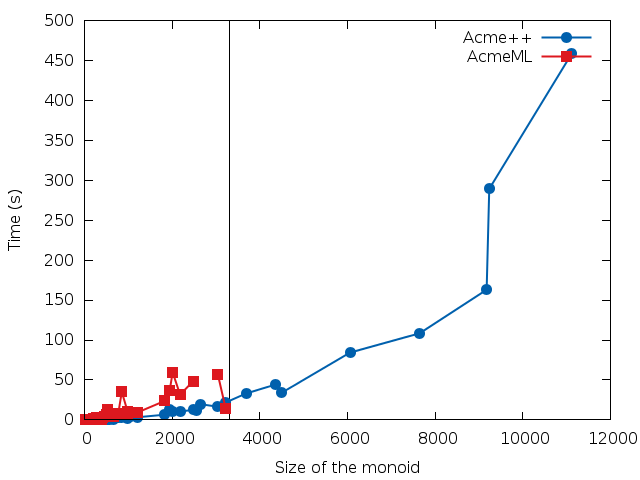
\includegraphics[width=0.8\textwidth]{graph/lines}
    \caption{The time it takes for the two implementations to
      calculate the Markov monoids generated by randomly picked
      automata of size 10}
  \end{center}  
\end{figure}

For all sizes $n$ of automata there is a threshold in the size of the
Markov monoid after which the AcmeML version will not be
practical. This threshold is expressed by the vertical line in the
example above. 

Even on smaller examples the Acme++ version outperforms AcmeML by a
large factor as seen in the following figure.

\begin{figure}
  \label{fig2}
  \begin{center}
    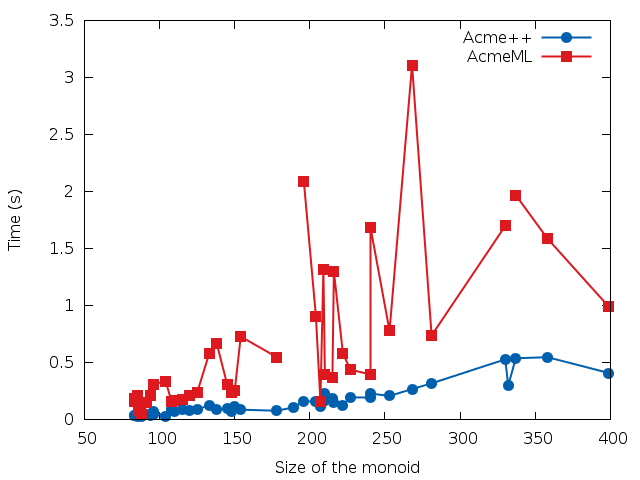
\includegraphics[width=0.8\textwidth]{graph/zoomlines}
    \caption{The same experiment as in fig.\ref{fig1} on automata
      generating smaller Markov monoids}
  \end{center}  
\end{figure}
